\section{SafeDE: a \underline{D}iversity \underline{E}nforcement hardware module}
\label{sec:dimmo}

This section presents the architecture of SafeDE, its features and limitations, its extension towards N-modular redundancy, and its implementation and integration (both hardware and software) details.

\subsection{SafeDE Architecture}
\label{sec:arch}

\begin{figure}[t!]
\centering
  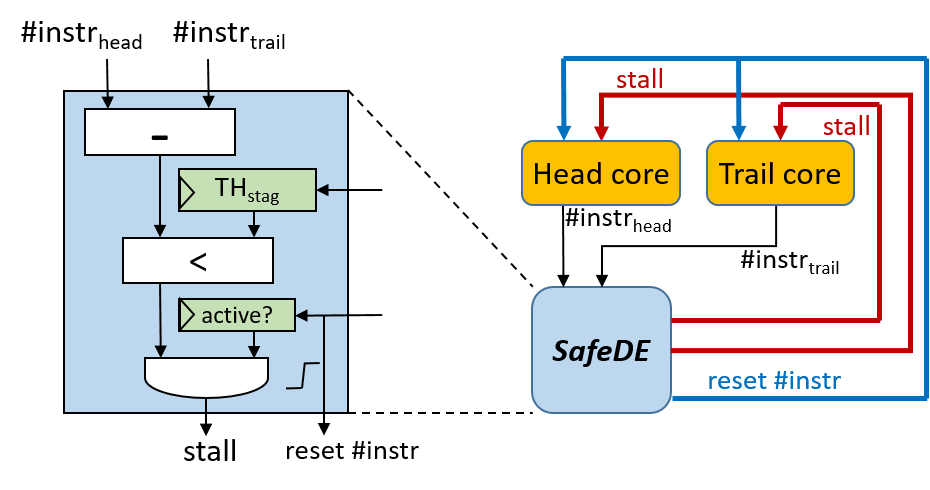
\includegraphics[width=1\columnwidth]{imgs/dimmo.png} 
  \caption{SafeDE architecture.}
  \label{fig:dimmo}
\end{figure}

SafeDE builds on the light-weight lockstepping concept, which has only been implemented in software so far~\cite{SergiDFT}, with the aim of preserving its advantages and removing its main limitations, i.e., the need for an extra core to run the monitor and a long feedback loop imposing a large staggering. SafeDE is architected as a tiny component connected to the two monitored cores, as shown in Figure~\ref{fig:dimmo}. SafeDE collects the instruction counts from the two cores, namely $\#instr_{head}$ and $\#instr_{trail}$, and generates the stall signal for the trail core. As for the software-only solution, SafeDE checks whether the head core is at least $TH_{stag}$ instructions ahead of the trail one. If this is not the case, the stall signal for the trail core is raised, which stalls its pipeline by stalling one or several of its stages (e.g., stalling the commit stage).

\textbf{SafeDE parameters}. The configuration registers of SafeDE are $TH_{stag}$, $active$, $CritSec1$ and $CritSec2$, and they operate as follows:
\begin{itemize}
\item $TH_{stag}$ corresponds to the minimum staggering (in terms of number of instructions) to be enforced between the head and trail cores. Typically, it has a very low value (e.g., 10 instructions), hence implementing a staggering distance much smaller than that of software-only solutions, and comparable to that of tight hardware-based lockstep execution.
\item $active$ determines whether SafeDE is active. If this signal is reset, SafeDE is completely neutral since it can never stall that trail core.
\item $CritSec1$ ($CritSec2$) is set by the head (trail) core when it enters the code region needing lockstep, and reset when leaving it. Hence, lockstepping must be enforced when $CritSec1$ and $CritSec2$ are both set, as this indicates that both cores are executing the code region needing lockstep execution.
\end{itemize}

\textbf{SafeDE operation}. While $active=0$, SafeDE is inactive. Eventually, $TH_{stag}$ is programmed and $active$ is set, hence activating SafeDE. Activating SafeDE automatically resets $CritSec1$ and $CritSec2$ keeping SafeDE ready but innocuous until $CritSec2$ is activated. Eventually, one of the two cores activates its $CritSec$ register, becomes the head core, and its instruction counter ($\#instr_{head}$) is reset and starts counting. Whenever the other core sets its $CritSec$ register, it becomes the trail core, and its instruction counter ($\#instr_{trail}$) is also reset. If the head core is not ahead $TH_{stag}$ instructions of the trail core, SafeDE sets the stall signal for the trail core. Note that, since any of the two cores could be the trail core depending on which one sets its $CritSec$ first, the $stall$ signal exists for both cores. Note that, if the staggering is too low when the trail core sets its $CritSec$ ($\#instr_{head} - \#instr_{trail} < TH_{stag}$), the $stall$ signal for the trail core will be raised immediately. Whenever the staggering is enough, the trail core is allowed to resume its execution.
Note that SafeDE checks every cycle whether the staggering is enough. This allows using tiny staggering ($TH_{stag}$) values, in contrast with the large staggering needed by the software-only solution. Moreover, SafeDE controls this condition, hence not needing any additional core to run any monitor software.
Also note that by performing such check every cycle, negligible switching power is induced since $\#instr_{head}$ and $\#instr_{trail}$ barely change.
Eventually, the head core reaches the end of its protected code region and resets its $CritSec$ register. At that point, SafeDE becomes innocuous again not raising any stall signal, hence letting the trail core reaching also the end of its protected region.

\textbf{Software process}. At software level, end users need to configure and set SafeDE active with the corresponding driver, and typically, use an API to schedule both redundant processes to the corresponding cores managing $CritSec$ registers accordingly. Those software components are described later in this section in the context of bare metal and Linux integrations.


\subsection{Features and Limitations Analysis}

This section presents the key features and limitations of SafeDE, and how they compare against the software-only solution~\cite{SergiDFT}. 

\subsubsection{SafeDE features}
\begin{itemize}
\item \textbf{Low cost}. SafeDE is a tiny hardware module implementing light-weight lockstep execution that avoids the need for an extra core to run a monitor at specific (tight) time intervals, as opposed to the software-only solution.
\item \textbf{Low staggering}. By controlling the feedback loop at hardware level, it is checked every cycle and hence, staggering can be kept to a minimum (e.g., 10 or 20 instructions). Note that the software-only solution needs a staggering value of many thousands of instructions to reach a staggering above 100$\mu$s, as discussed before.
\item \textbf{Flexibility}. SafeDE can be easily enabled and disabled. Hence, the main overheads relate to the creation of the redundant processes at software level, as needed in the context of light-weight lockstep execution, but not to the actual implementation of SafeDE, which does not impose further limitations.
\item \textbf{Low intrusiveness}. SafeDE needs some signals to be exported from cores, such as those to read and reset instruction counts, and the pipeline stalling signal. These modifications are much lighter than those needed in the case of tight lockstep execution. While the software-only solution does not require any hardware change, as opposed to SafeDE, it may need modifying the operating system to enable the management of the instruction counts remotely from other cores. SafeDE does not need any such operating system modification.
\end{itemize}

\subsubsection{SafeDE limitations}
\begin{itemize}
\item \textbf{Non-null intrusiveness}. While hardware modifications needed by SafeDE are light, it needs hardware support, and hence, cannot be used on COTS multicores, as opposed to the software-only solution.
\item \textbf{Limited applicability}. Light-weight lockstepping relies on the redundant processes executing identical instruction streams to guarantee the effectiveness of the approach. While this is usually the case, it precludes the use of this scheme for programs whose control path is non-deterministic (e.g., based on random choices independent across redundant processes). 
Also, SafeDE may not be used for parallel programs if the number of instructions of any thread may vary depending on the order in which they get a specific lock, since this could make redundant threads execute a different number of instructions. 
Also, since light-weight lockstepping exposes all activity redundantly, it should not be used along with I/O operations that may change the functionality of the system if repeated. In any case, note that those limitations relate to the light-weight lockstepping scheme rather than to SafeDE, and hence, affect also the software-only solution.
\item \textbf{Limited diversity}. By using two cores with staggered execution, SafeDE, as well as the software-only solution, provide physical and time diversity. However, if CCFs can be induced by the core design (e.g., physically weak gates identical in both cores), other types of diversity, such as layout diversity, are needed, and such diversity cannot be reached without appropriate (and intrusive) hardware modifications.
\item \textbf{SafeDE hardening}. SafeDE must be hardened to mitigate the risk of a single fault in SafeDE leading to a failure. Alternatively, SafeDE can also be implemented with physical diverse redundancy, as for tight lockstepping replicating the scheme in Figure~\ref{fig:HWSWlockstep}(a), but applied to SafeDE instead of to the cores.
\end{itemize}

\subsubsection{Scope of applicability}
As discussed before, light-weight lockstepping has limited applicability, hence affecting both SafeDE and the software-only solution. Therefore, SafeDE can only be used for some code regions rather than for the full program. Code regions exercising light-weight lockstepping limitations must be run on cores implementing tight lockstepping. Hence, at least two cores must implement tight hardware-based lockstepping. However, compute intensive parts of the code can be managed with SafeDE. This opens the door to using deployments with two tightly lockstepped cores (e.g., to run I/O-related code regions) and the remaining cores building on SafeDE. For instance, an 8-core multicore would offer 7 user-visible cores by shadowing only one of the cores for tight lockstepping. Hence, one could run a varying number of lockstepped and non-lockstepped tasks, ranging from 4 lockstepped to 1 lockstepped and 6 non-lockstepped. Instead, if tight lockstepping is used for all cores, then only 4 cores are visible at user level regardless of whether tasks need such support.

\subsection{Towards N-modular Redundancy}

\begin{figure}[t!]
\centering
  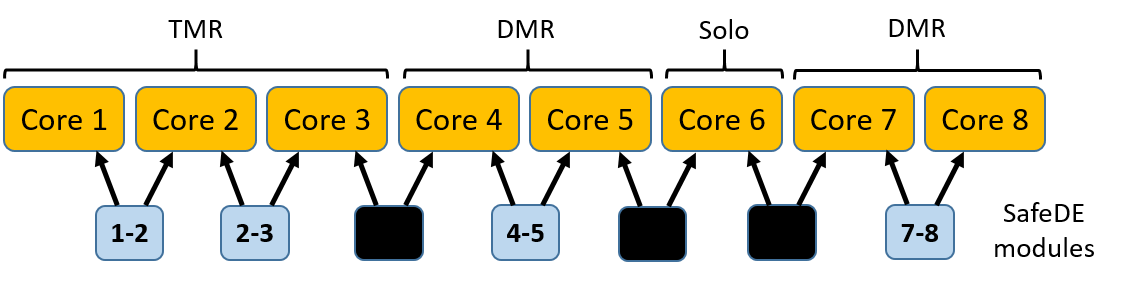
\includegraphics[width=1\columnwidth]{imgs/Nmodular.png} 
  \caption{N-modular redundancy scheme example with SafeDE.}
  \label{fig:Nmodular}
\end{figure}


Note that, while we implement and assess SafeDE in the context of dual-modular redundancy (DMR), it can be easily extended to N-modular redundancy, which may be needed for $N>2$ in some domains such as, for instance, avionics or medical, where 3-modular or even 5-modular redundancy may be needed. 

Regardless of the value of $N$, SafeDE must manage the $N$ cores so that one of them is the head core, one of them is the trail core, and the remaining ones inherit both, head and trail behavior. For instance, in the case of triple-modular redundancy (TMR), core 1 is the head core w.r.t. core 2, core 2 is the trail core w.r.t. core 1 and the head core w.r.t. core 3, and core 3 is the trail core w.r.t. core 2.
Therefore, given $N$ cores, SafeDE must activate the $stall_i$ signal for $core_i$ if the following condition holds: $\#instr_{i-1} - \#instr_{i} < TH_{stag}$, where $\#instr_{i-1}$ and $\#instr_i$ correspond to the instruction counts of $core_{i-1}$ and $core_i$ respectively, and $1 \le i < N$.

In the context of N-modular redundancy, note that the operation with $CritSec$ is analogous to DMR, hence cores take the role of $core_i$ when they are the $i^{th}$ core setting their corresponding $CritSec$ register. A core $core_i$ cannot be further stalled when $core_{i-1}$ leaves its critical region by resetting its $CritSec$ register. However, the remaining cores (from $core_{i+1}$ to $core_{N}$) can still be stalled if their staggering becomes too low w.r.t. their respective head cores.

One potential realization of the overall concept with flexible N-modular redundancy could impose that the cores in the multicore are physically paired for SafeDE operation so that $core_1$ is the head of $core_2$, $core_2$ of $core_3$, and so on and so forth. Then, $N-1$ SafeDE modules are deployed connecting each pair of consecutive cores. Finally, by activating appropriate SafeDE modules, one could have any combination of N-modular redundancy at will. For instance, Figure~\ref{fig:Nmodular} illustrates a case where an 8-core multicore uses 3 cores with TMR (cores 1-3), two pairs of 2 cores with DMR (cores 4-5 and 7-8), and 1 core running independently (core 6). This is achieved by enabling specific SafeDE modules (light-colored ones) and keeping others inactive (black ones).



\subsection{Implementation and Integration}
\label{sec:integ}

\begin{figure}[t!]
\centering
  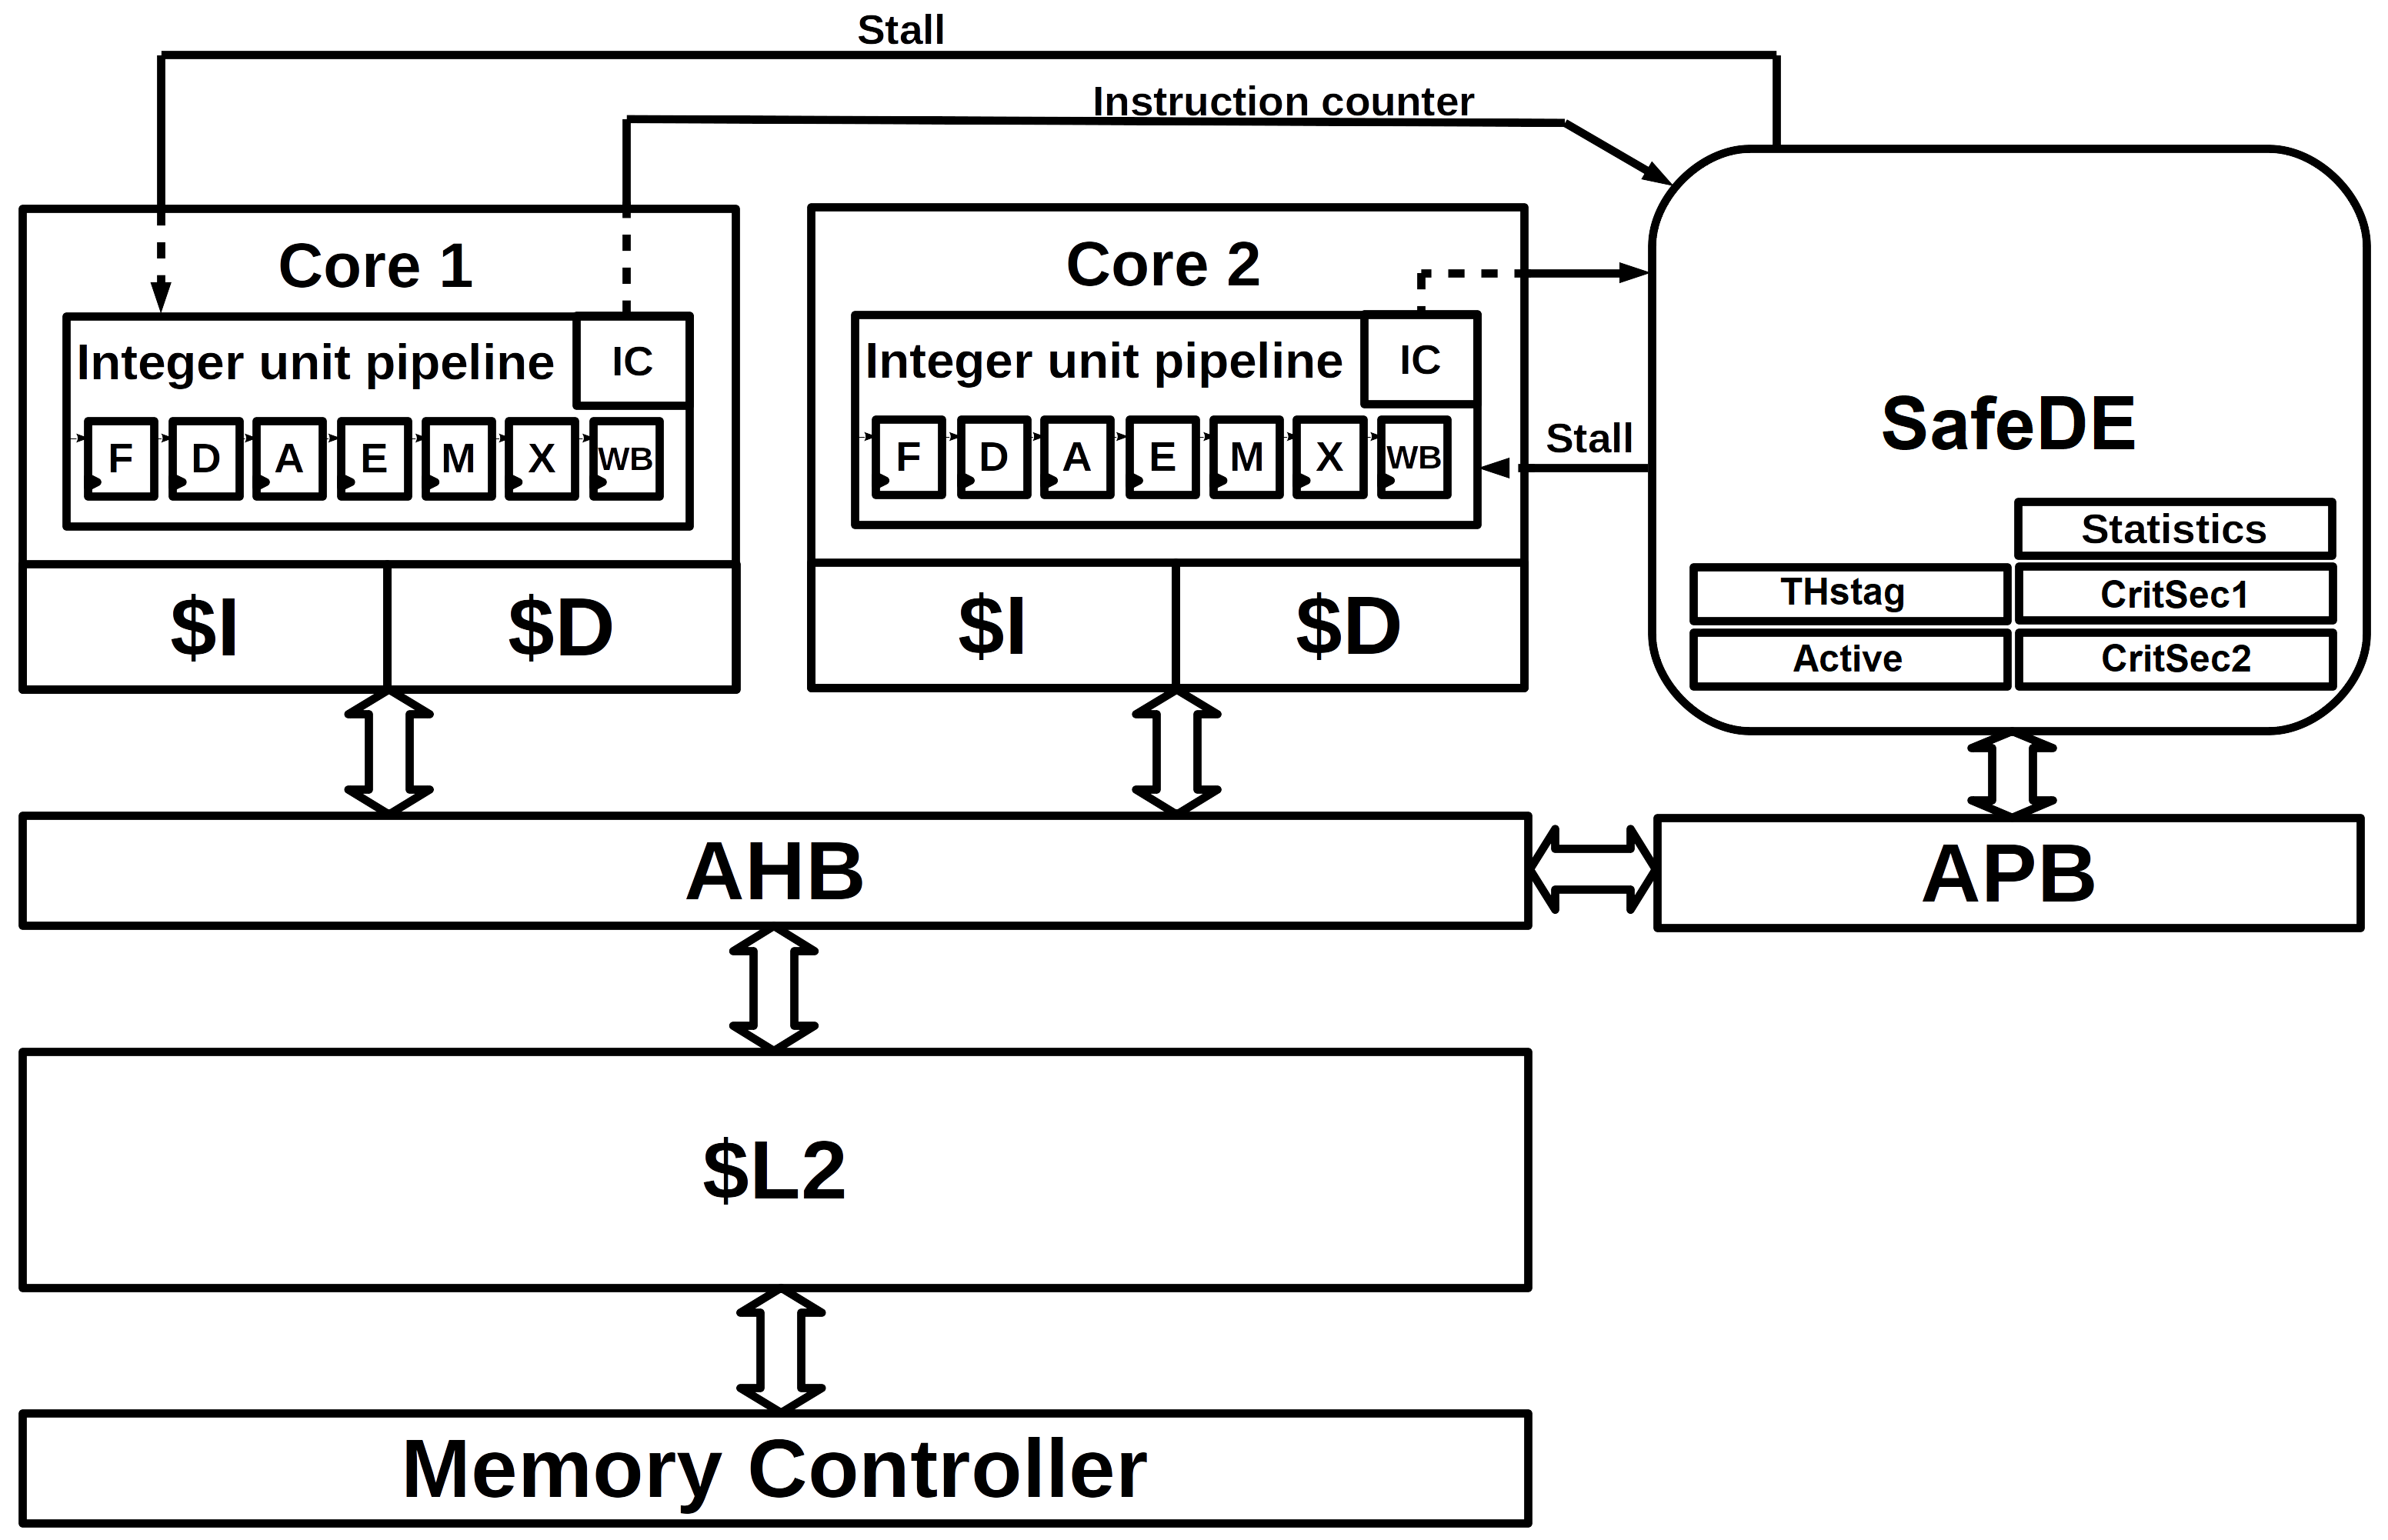
\includegraphics[width=1\columnwidth]{imgs/system.png} 
  \caption{High-level representation of SafeDE integrated into the system.}
  \label{fig:system}
\end{figure}

As a proof of concept, we have integrated SafeDE in an industrial space MultiProcessor System on Chip (MPSoC) based on CAES Gaisler RISC-V NOEL-V cores~\cite{SELENEgit}. This platform consists of a consistent set of reusable VHDL IP cores by Gaisler whose main interface is a set of common on-chip buses. Those buses implement the standard AMBA 2.0, and SafeDE has been implemented in VHDL as another IP core compatible with such bus interface.

\subsubsection{System on Chip}
SafeDE is integrated and evaluated in a specific MPSoC instance including 2 Gaisler's NOEL-V 64-bit cores. Those cores are dual-issue, implement the RISC-V Instruction Set Architecture (ISA), include 7 pipeline stages, and local L1 data and instruction caches. Cores are connected among them, and to a shared L2 cache and the memory subsystem through a 128-bit AMBA Advanced High-performance Bus (AHB). Components requiring low bandwidth, such as for instance, SafeDE, are connected instead through an AMBA Advanced Peripheral Bus (APB).

\subsubsection{Hardware integration}
SafeDE interface builds on the standard APB interface to make it highly portable. In particular, SafeDE is an APB slave in the SoC.
SafeDE is also directly connected to the cores to collect their instruction counters, which are mapped to SafeDE as inputs, to stall the trail core whenever needed. The instruction counters determine the number of instructions executed by each core and used to compute the real staggering across head and trail cores. Regarding the stall signal produced by SafeDE, it is ORed with an internal core signal in charge of freezing the pipeline by not allowing register values to be updated. Overall, the only modifications needed in the cores include exporting the instruction counter\footnote{Note that the instruction counter, along with the cycle counter, are the main counters in any processor and are generally implemented in any SoC.} to SafeDE, and placing an OR gate appropriately to stall the pipeline whenever needed.
The SoC including SafeDE is depicted in Figure \ref{fig:system} for completeness.

\subsubsection{Configuration and operation}
SafeDE configuration registers, namely $TH_{stag}$, $active$, $CritSec1$ and $CritSec2$, are mapped to specific memory addresses. Their operation is detailed in Section~\ref{sec:arch}.
Apart from those functional registers, SafeDE also includes several statistics registers collecting information such as the maximum and minimum staggering observed, number of stall signal activations (i.e., how many times the $stall$ signal is raised), number of stall cycles for the trail core, executed instructions of each core, etc. 
Since SafeDE has an APB interface and memory-mapped registers, all its registers can be read and written with regular load and store operations.

\subsection{Software Integration}

We have developed the software interface to control the SafeDE IP. We considered two scenarios where SafeDE can be deployed: bare-metal systems, and systems with an operating system (Linux in our case). Hence, we implemented two software integrations. A C library, which is enough for a bare metal setup, and a driver for a Linux setup.

\subsubsection{Bare Metal Integration}
\label{sec:bare_metal}

To integrate SafeDE software in a bare metal setup we have created an API that consists of a C library to configure the internal SafeDE registers. The API contains functions to enable and reset SafeDE, configure the staggering, indicate when the critical section starts and finishes for each core, and gather the execution results (statistics).
At run time, SafeDE must be initialized first.
Such initialization includes configuring the staggering, and setting the reset and enable bits using the API. Whenever a core starts or finishes the critical region, a function from the API has to be executed to notify the SafeDE module. Once the task has finished, the statistics from the safe execution can be retrieved, again, using a function provided in the API library.

\subsubsection{Linux Integration}

In Linux, it is not possible to access directly the memory positions mapped to SafeDE registers from the user space. To allow the user to access SafeDE registers, we need to access the kernel space using a driver. We have programmed a Linux driver and a C library (API) that allow the user to communicate with the SafeDE module. 

For the Linux API, we use a set of functions analogous to those for the bare metal integration, but this time managed through the driver. The API calls communicate with the driver by writing the commands into a Linux device file, a special file in the Linux file system created during the driver initialization process. Later, the driver reads the commands from the device file and modifies the SafeDE registers accordingly. 

As stated before, one of the SafeDE limitations is that both cores have to execute the exact same instructions. However, in a preemptive operating system, a process in the critical region may be preempted. Since the critical region is active, instructions executed in that core would be counted as part of the critical region, hence de-synchronizing staggering in an arbitrary manner. Deactivating the corresponding $CritSec$ register would not be a better solution since it would not occur immediately, hence altering the instruction count anyway, and would lead to the virtual finalization of the lockstep execution. 
Some guidelines to avoid this situation are as follows:
\begin{enumerate}
    \item In Linux, each process has a mask indicating in which subset of the cores that process can be executed (a.k.a. process affinity). The particular case in which this subset is only one core, is named binding. In our strategy, we bind the two critical processes into two cores and modify all the other processes (including kernel processes) affinity to avoid preemption of the critical processes.
    \item In order to give the highest priority to the two redundant critical tasks so that they start immediately and unnecessary stalls do not occur, we must enqueue those tasks into the highest priority queue, which is SCHED\_FIFO queue. We perform that employing the Linux system call \textit{sched\_setscheduler()}. 
\end{enumerate}


Note that, if a real-time operating system (RTOS) for safety-related systems was used instead of Linux (e.g., fentISS' XtratuM, SYSGO's PikeOS, RTEMS), such problem would not exist and simpler mechanisms related to task scheduling and priority assignment would suffice to guarantee the non-preemptive execution of light-weight lockstepped processes.


